\begin{question}
    \normalfont


    Let $A$ be the $2\times2$ matrix given by
    \begin{align*}
        A = \MatrixTwoTwo{a}{b}{c}{d}.
    \end{align*}
    Let $B_i$ be the matrices given by
    \begin{align*}
        B_1 = \MatrixTwoTwo{0}{1}{1}{0},\ \ \
        B_2 = \MatrixTwoTwo{\cos\theta}{-\sin\theta}{\sin\theta}{\cos\theta},\ \ \
        B_3 = \MatrixTwoTwo{1}{0}{5}{1},\ \ \
        B_4 = \MatrixTwoTwo{2}{0}{0}{3}.
    \end{align*}
    For each of the $B_i$ matrices, above, complete the following:
    \begin{enumerate}[(i)]
        \item compute $B_iA$;
        \item draw a picture of $\real^2$, showing $e_1, e_2$ and $B_ie_1, B_ie_2$, and describe what has changed geometrically from the list $[e_1, e_2]$ to $[B_ie_1, B_ie_2]$;
        \item compute $\det(B_iA)$ in terms of the value of $\det(A)$.  (You are meant to do this calculation directly, from the definition of $2\times2$ determinant. Do not invoke the properties of determinant, such as LADW Theorem 3.5.)
    \end{enumerate}
\end{question}
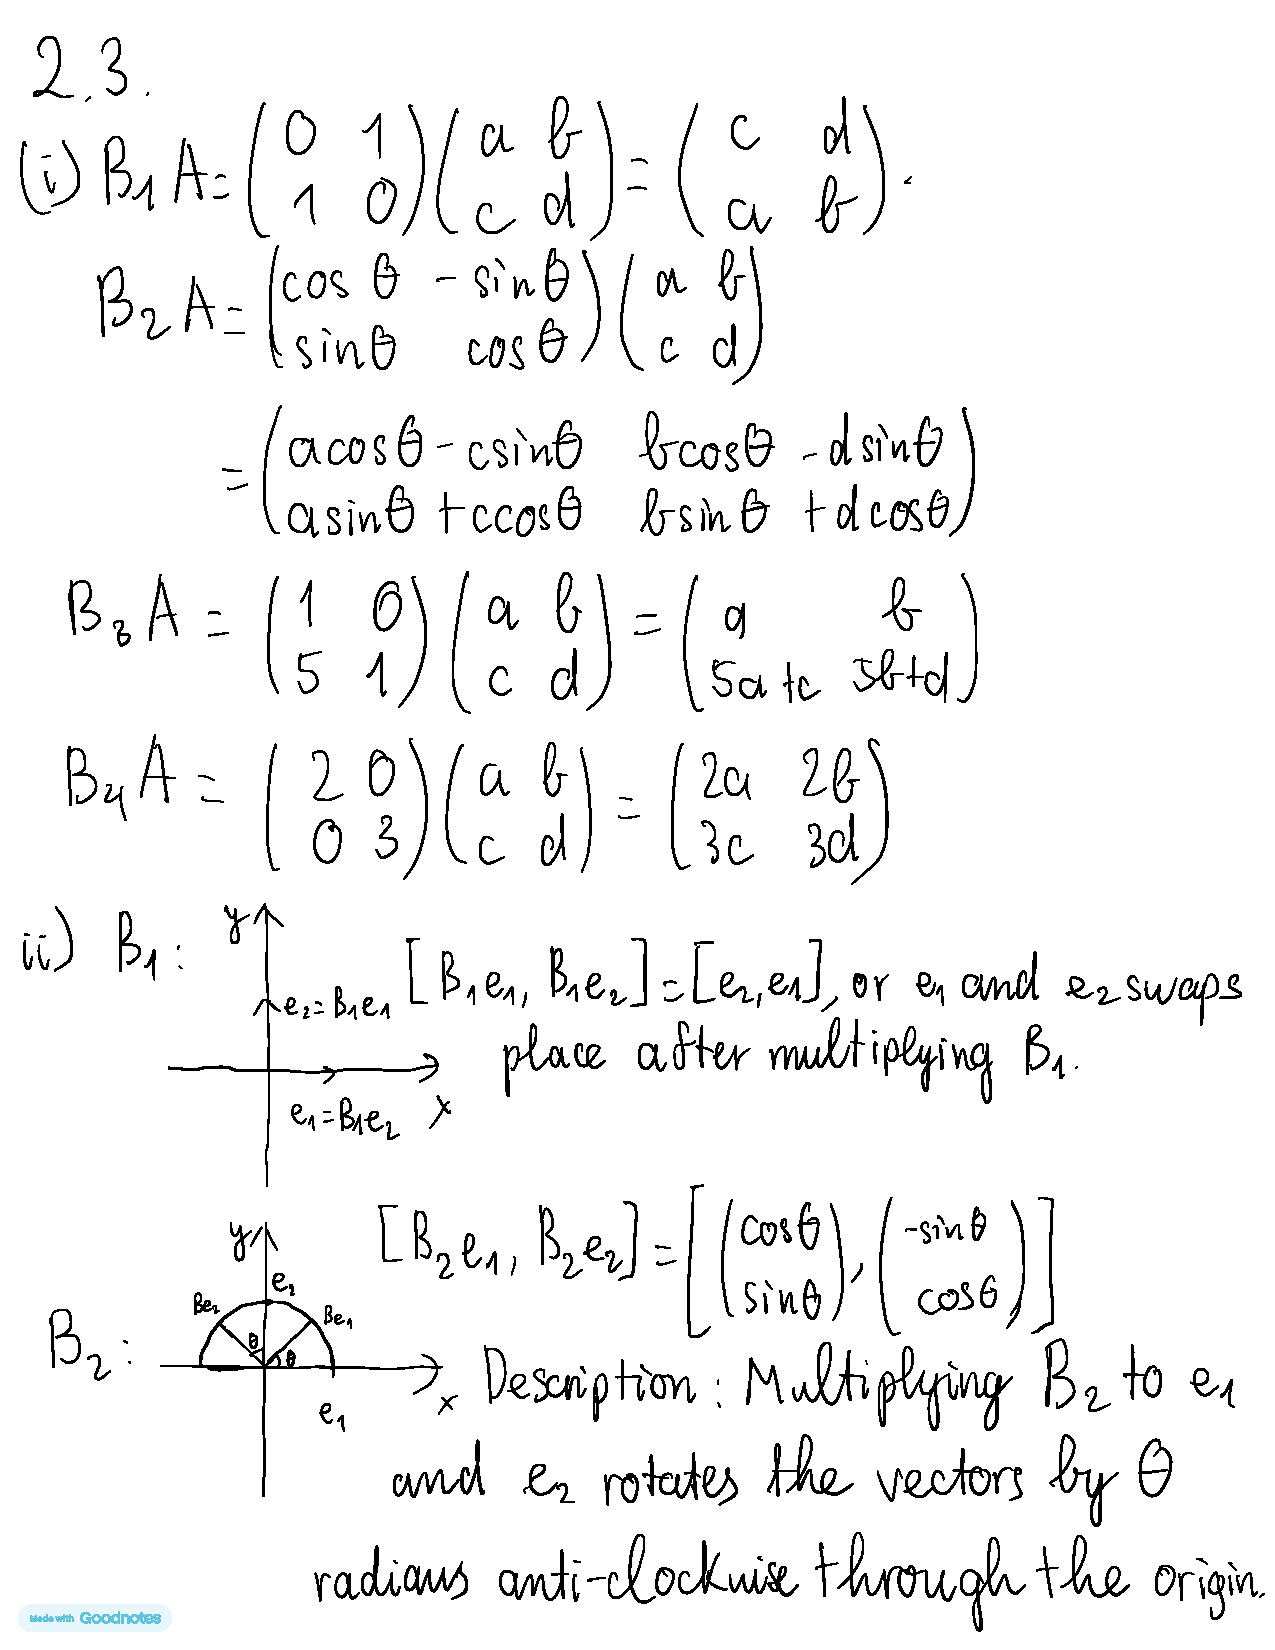
\includepdf[pages=-]{2.3.pdf}